% !TeX root = ../dd.tex

The following chapter aims to show the strategies implemented in order to better integrate and test the various components. The main purpose of the tests conducted is to try to induce and recreate, as early as the development phase, situations that might give rise to malfunctions or inate behaviors, so that they can be resolved before the final version intended for the public.


\section{Feature Identification}

\begin{table}[H]
    %\caption*{\textbf{Title}}
    \centering
    \begin{tabular}{|l|l|l|}
        \hline
        \textbf{Feature}                    & \textbf{Importance} & \textbf{Difficulty} \\\hline
        Login                               & High                & Medium              \\
        AI CV Generation   & High                & High                 \\
        Publish internship ADV & High                & Low              \\
        Custom notification & Medium                & High                \\
        Send reports        & High                & Low                 \\
        Chat                & Low              & High                 \\
        AI Homepage Feed    & High              & Low               \\\hline
    \end{tabular}
    \caption{Importance and difficulty of features}
    \label{table:Importance and difficulty of features}
\end{table}

\section{Development and Test Plan}
The components were developed using a bottom-up approach, so that the work could be divided into several independent parts, each assigned to a different team. Subsequently, after completing the equal parts as well as those of high importance, we began to integrate them into the system, as described below.
The tests were divided into the following categories: 
\begin{itemize}
    \item \textbf{Functional Testing} - in order check the presence of bugs.
    \item \textbf{Performance Testing} - in other to check if the system is responsive.
    \item \textbf{Stress Testing} - in order to simulate intensive use in a real-world scenario
\end{itemize}

\section{Component integration and testing}
The following section shows how the individual components were implemented in the system.
In the following section ne interaction between components are shown using graphs.

\subsection{Login}
The only part that need to be tested is the interaction of the system with the interfaces
provided by the two different authentication method (via OAuth2 for companies and via eduGAIN radius connection for students). The authentication services used are considered reliable by definition. 

\begin{figure}[H]
    \centering
    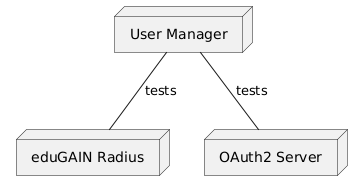
\includegraphics[width=0.5\textwidth]{dd/assets/componen-itntegration-diagram/1-login.png}
    \caption{User manager.}
    \label{fig:User manager}
\end{figure}

\subsection{Platform Manager}
This component, in addition to allowing automatic CV generation, enables the addition of new job offers.
For this purpose, given the criticality and confidentiality of the information contained, it was decided not to use external services, so all CVs are generated within the Platform Manager.

\begin{figure}[H]
    \centering
    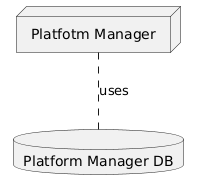
\includegraphics[width=0.3\textwidth]{dd/assets/componen-itntegration-diagram/2-platform-manager.png}
    \caption{Platform manager.}
    \label{fig:Platform manager}
\end{figure}

\subsection{Relation Manager}

\begin{figure}[H]
    \centering
    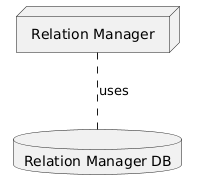
\includegraphics[width=0.3\textwidth]{dd/assets/componen-itntegration-diagram/3-relation-manager.png}
    \caption{Relation manager.}
    \label{fig:Relation manager}
\end{figure}

\subsection{Recommendation Manager}
\begin{figure}[H]
    \centering
    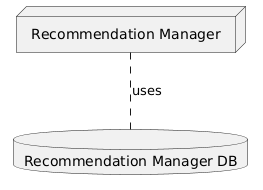
\includegraphics[width=0.3\textwidth]{dd/assets/componen-itntegration-diagram/4-recommendation-service.png}
    \caption{Relation manager.}
    \label{fig:Relation manager}
\end{figure}

\subsection{Notification Manager}
\begin{figure}[H]
    \centering
    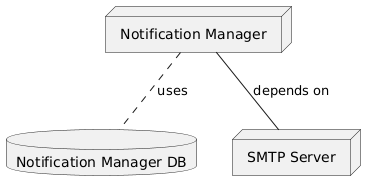
\includegraphics[width=0.5\textwidth]{dd/assets/componen-itntegration-diagram/5-notification-manager.png}
    \caption{Notification manager.}
    \label{fig:Notification manager}
\end{figure}

At this point all subsystems have been implemented and tested, so the next step is per-
forming integration testing between the subsystems and the API Gateway

\begin{figure}[H]
    \centering
    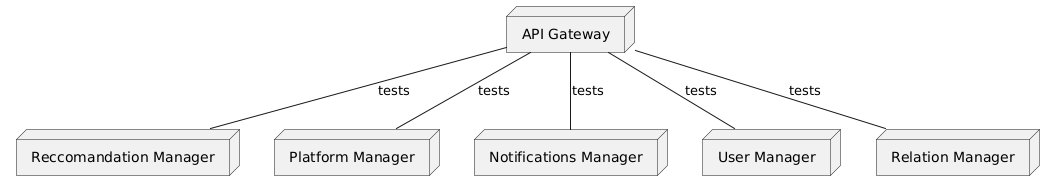
\includegraphics[width=0.8\textwidth]{dd/assets/componen-itntegration-diagram/api-gateway.png}
    \caption{API Gateway}
    \label{fig:API Gateway}
\end{figure}

Since all the mangers have few iterations between them, except for the notification manager, the testing phase was carried out in a very focused mode on individual components.

Therefore, the only iterations tested separately were with the “Notification Manager” component and the interaction between “Relation Manager” and “Platform Manager” upon receipt of internship interruption request.

\begin{figure}[H]
    \centering
    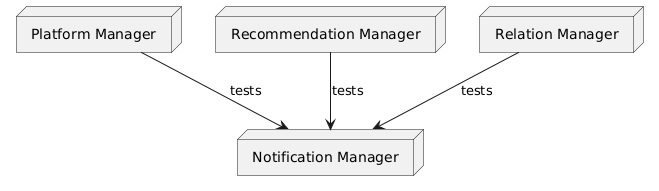
\includegraphics[width=0.8\textwidth]{dd/assets/componen-itntegration-diagram/tests/1-notification-test.png}
    \caption{Notification manager tests.}
    \label{fig:Notification manager tests}
\end{figure}

\begin{figure}[H]
    \centering
    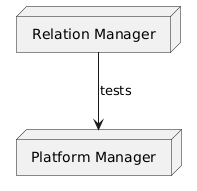
\includegraphics[width=0.3\textwidth]{dd/assets/componen-itntegration-diagram/tests/2-relation-platform.png}
    \caption{Testing between the “Relation Manager” and the “Platform Manager”.}
    \label{fig:Testing between the “Relation Manager” and the “Platform Manager”}
\end{figure}

\pagebreak
